\hypertarget{framework}{%
\section{\texorpdfstring{\href{http://en.wikipedia.org/wiki/Software_framework}{Framework}}{Framework}}\label{framework}}

\begin{itemize}
\tightlist
\item
  Fonctionnalités similaires pour de nombreuses applis
\item
  Composants de haut-niveau réutilisables (faible couplage)
\item
  Règles de codage et d'architecture
\item
  Code sûr et efficace
\item
  Facilite les tests et la gestion de projets complexes
\item
  Utilisation de Design Patterns dès que possible
\item
  Comportement par défaut
\item
  Extensible
\item
  Principe d'inversion de contrôle
\end{itemize}

Différences entre framework et library sur
\href{http://stackoverflow.com/questions/148747/what-is-the-difference-between-a-framework-and-a-library}{Stack
Overflow} ou
\href{http://www.artima.com/forums/flat.jsp?forum=106\&thread=152104}{artima
developper}.

\#Design Patterns et webdev

\begin{itemize}
\tightlist
\item
  Inversion de contrôle
  (\href{http://martinfowler.com/bliki/InversionOfControl.html}{IoC})
\item
  Model View Controller

  \begin{itemize}
  \tightlist
  \item
    M : Accès aux données, logique métier
  \item
    V : Templates des pages à générer
  \item
    C : Orchestration, transfert des infos
  \end{itemize}
\item
  Front Controller

  \begin{itemize}
  \tightlist
  \item
    Traitement et dispatch des requêtes
  \item
    (bootstrap, ré-écriture des URL, \ldots{})
  \end{itemize}
\item
  \href{http://blog.mazenod.fr/2010/01/design-pattern-mvc-zoom-sur-la-couche-modele-dal-dao-orm-crud/}{Object
  Relational Mapping}

  \begin{itemize}
  \tightlist
  \item
    Active Record, Table Data Gateway, Data Mapper, \ldots{}
  \end{itemize}
\item
  \href{http://ui-patterns.com/}{UI Patterns}
\end{itemize}

\hypertarget{mvc-for-webdev}{%
\section{MVC for webdev}\label{mvc-for-webdev}}

\begin{figure}
\centering
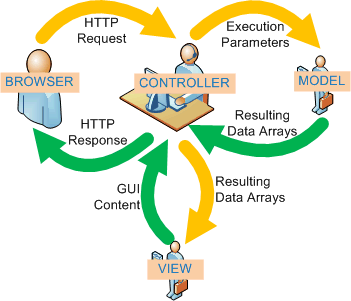
\includegraphics{src/img/mvc.png}
\caption{``MVC''}
\end{figure}

\hypertarget{conventions}{%
\section{Conventions}\label{conventions}}

\begin{itemize}
\tightlist
\item
  Nommage

  \begin{itemize}
  \tightlist
  \item
    Classes
  \item
    Base de données
  \item
    Fichiers et dossiers
  \end{itemize}
\item
  ROUTES :
  \begin{otherlanguage}{english}\texttt{http://app.host.tld/controller/action{[}/key/val{]}}\end{otherlanguage}
\item
  Arborescence :

  \begin{itemize}
  \tightlist
  \item
    Imposée ou libre selon frameworks
  \item
    Pas de code (minimum) sous la racine web
  \end{itemize}
\item
  Conventions obligatoires ou non, mais RECOMMANDEES dans tous les cas
\end{itemize}

\hypertarget{bonnes-pratiques}{%
\section{Bonnes pratiques}\label{bonnes-pratiques}}

\begin{itemize}
\tightlist
\item
  Heavy Model, Light Controller
\item
  Don't Repeat Yourself
\item
  You Ain't Gonna Need It
\item
  Convention Over Configuration
\item
  Keep It Simple and Stupid
\item
  \href{https://12factor.net/}{12 factor app} -
  \href{https://12factor.net/fr/}{fr}
\end{itemize}

\hypertarget{pretty-smart-clean-formatted-url}{%
\section{Pretty ( \textbar{} smart \textbar{} clean \textbar{}
formatted) URL}\label{pretty-smart-clean-formatted-url}}

\begin{itemize}
\tightlist
\item
  Les URL doivent être explicites :

  \begin{itemize}
  \tightlist
  \item
    Manipulées par l'utilisateur
  \item
    Utilisées pour le référencement
  \end{itemize}
\item
  Cohérence avec l'implémentation MVC :
\end{itemize}

\begin{otherlanguage}{english}

\begin{verbatim}
http://app.host.tld/controller/action[/key/val]
\end{verbatim}

\end{otherlanguage}

\begin{itemize}
\tightlist
\item
  Le routage (routing)

  \begin{itemize}
  \tightlist
  \item
    Le Front Controller recoit toutes les requêtes (URL rewriting)
  \item
    Il les dispatche vers les contrôleurs
  \end{itemize}
\end{itemize}

\hypertarget{smart-url-seo}{%
\section{Smart URL \& SEO}\label{smart-url-seo}}

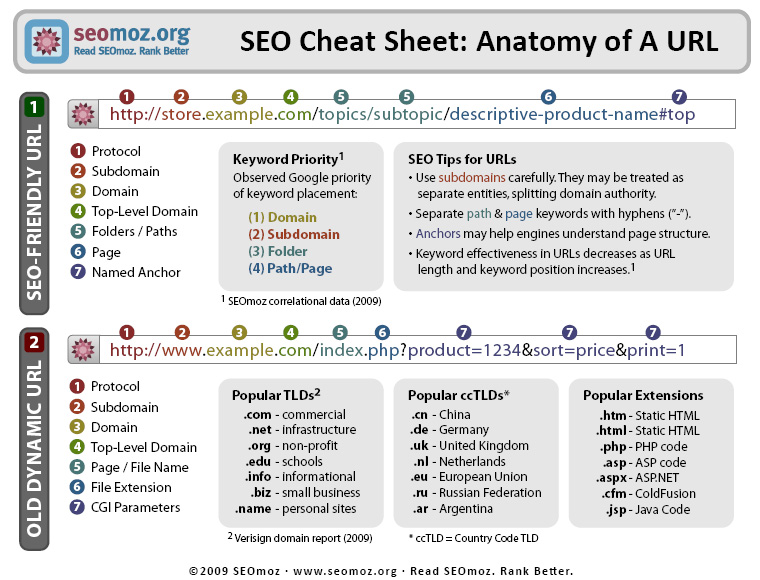
\includegraphics{src/img/anatomy-of-a-url.jpg}

\hypertarget{autres-services}{%
\section{Autres Services}\label{autres-services}}

\begin{itemize}
\tightlist
\item
  Migrations : Evolutions de la strucutre de la BDD
\item
  Tests
\item
  Génération, validation et traitement de formulaires
\item
  Authenfication, Sessions, Permissions, Roles, ACL
\item
  Pagination
\item
  I18n
\item
  Génération de code
\item
  Mail
\item
  Connecteurs aux webservices
\item
  Captchas
\item
  Loggers
\item
  \ldots{}
\end{itemize}

\hypertarget{exemple-darchitecture-laravel}{%
\section{Exemple d'architecture :
Laravel}\label{exemple-darchitecture-laravel}}

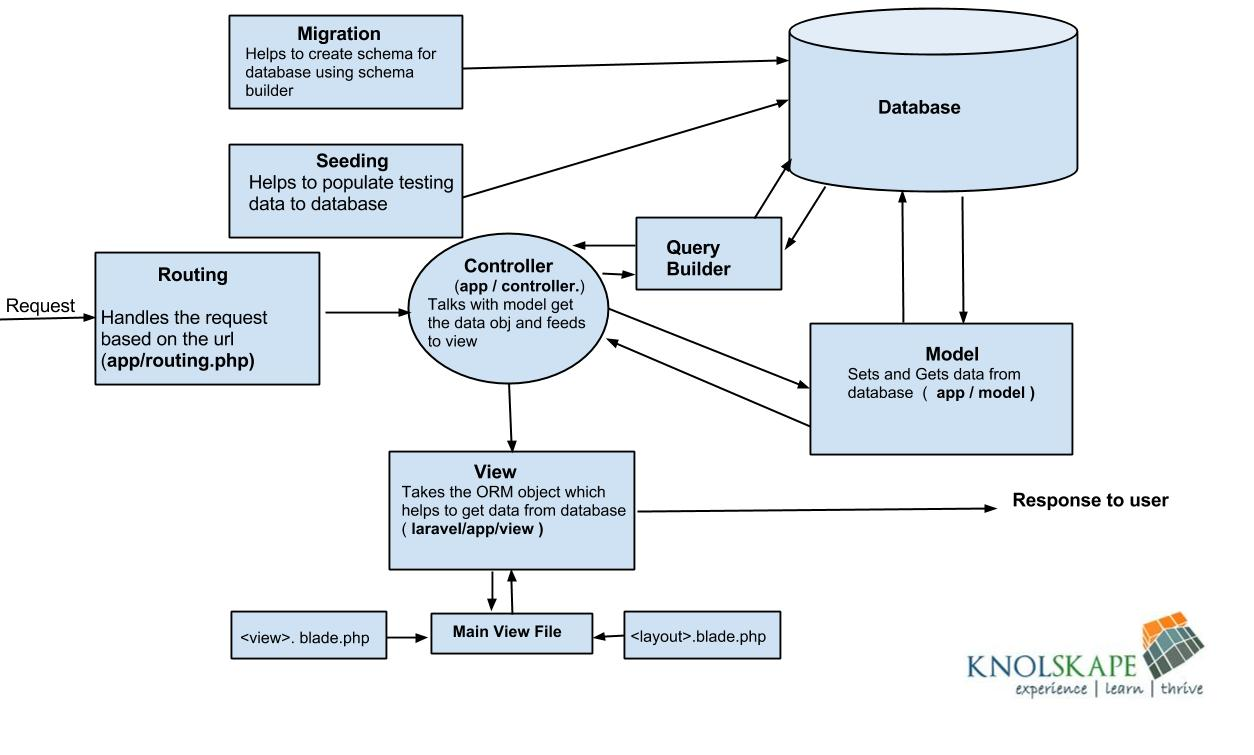
\includegraphics{src/img/laravel-architecture.jpg}

\hypertarget{performance}{%
\section{Performance}\label{performance}}

\begin{itemize}
\tightlist
\item
  Un framework web est lent :

  \begin{itemize}
  \tightlist
  \item
    Rendu d'une page nécéssite de traverser tout le code
  \item
    Pour chaque requête toute l'appli est chargée
  \item
    Plus de code qu'une appli standalone
  \item
    Plus de requêtes
  \end{itemize}
\item
  Solutions

  \begin{itemize}
  \tightlist
  \item
    Cache de pages, d'opcode
  \item
    Jointures ORM, vues, procédures stockées
  \item
    Outils d'optimisation : YSlow, page speed, mytop \# Sources
  \end{itemize}
\end{itemize}
